\documentclass[11pt]{scrartcl}
\usepackage[T1]{fontenc}
\usepackage[a4paper, left=3cm, right=2cm, top=2cm, bottom=2cm]{geometry}
\usepackage[activate]{pdfcprot}
\usepackage[ngerman]{babel}
\usepackage[parfill]{parskip}
\usepackage[utf8]{inputenc}
\usepackage[math]{kurier}
\usepackage{amsmath}
\usepackage{amssymb}
\usepackage{xcolor}
\usepackage{epstopdf}
\usepackage{txfonts}
\usepackage{fancyhdr}
\usepackage{graphicx}
\usepackage{prettyref}
\usepackage{hyperref}
\usepackage{eurosym}
\usepackage{setspace}
\usepackage{units}
\usepackage{eso-pic,graphicx}
\usepackage{icomma}
\usepackage{pdfpages}

\definecolor{darkblue}{rgb}{0,0,.5}
\hypersetup{pdftex=true, colorlinks=true, breaklinks=false, linkcolor=black, menucolor=black, urlcolor=darkblue}



\setlength{\columnsep}{2cm}


\newcommand{\arcsinh}{\mathrm{arcsinh}}
\newcommand{\asinh}{\mathrm{arcsinh}}
\newcommand{\ergebnis}{\textcolor{red}{\mathrm{Ergebnis}}}
\newcommand{\fehlt}{\textcolor{red}{Hier fehlen noch Inhalte.}}
\newcommand{\betanotice}{\textcolor{red}{Diese Aufgaben sind noch nicht in der Übung kontrolliert worden. Es sind lediglich meine Überlegungen und Lösungsansätze zu den Aufgaben. Es können Fehler enthalten sein!!! Das Dokument wird fortwährend aktualisiert und erst wenn das \textcolor{black}{beta} aus dem Dateinamen verschwindet ist es endgültig.}}
\newcommand{\half}{\frac{1}{2}}
\renewcommand{\d}{\, \mathrm d}
\newcommand{\punkte}{\textcolor{white}{xxxxx}}
\newcommand{\p}{\, \partial}
\newcommand{\dd}[1]{\item[#1] \hfill \\}

\renewcommand{\familydefault}{\sfdefault}
\renewcommand\thesection{}
\renewcommand\thesubsection{}
\renewcommand\thesubsubsection{}


\newcommand{\themodul}{Optische Technologie}
\newcommand{\thetutor}{Prof. Rateike}
\newcommand{\theuebung}{Formelsammlung OT 2015}

\pagestyle{fancy}
\fancyhead[L]{\footnotesize{C. Hansen}}
\chead{\thepage}
\rhead{}
\lfoot{}
\cfoot{}
\rfoot{}

\title{ \theuebung{}}


\author{Christoph Hansen \\ {\small \href{mailto:chris@university-material.de}{chris@university-material.de}} }

\date{}


\begin{document}

\maketitle

Dieser Text ist unter dieser \href{http://creativecommons.org/licenses/by-nc-sa/4.0/}{Creative Commons} Lizenz veröffentlicht.

\textcolor{red}{Ich erhebe keinen Anspruch auf Vollständigkeit oder Richtigkeit. Falls ihr Fehler findet oder etwas fehlt, dann meldet euch bitte über den Emailkontakt.}

\tableofcontents


\newpage


\section{Linsen}

\subsection*{Allgemein}

\begin{align*}
\frac{1}{f} &= \frac{1}{b} + \frac{1}{g}  \\
m &= - \frac{b}{g}
\intertext{Linsenschleiferfromel für dünne Linsen:}
\frac{1}{f} &= \left( n - 1 \right) \cdot \left( \frac{1}{r_1} - \frac{1}{r_2} \right)
\intertext{Linsenschleiferfromel für dicke Linsen:}
\frac{1}{f} &= \left( n - 1 \right) \cdot \left( \frac{1}{r_1} - \frac{1}{r_2}  + \frac{(n - 1) \cdot d}{r_1 \cdot r_2 \cdot n}\right)
\end{align*}

\subsection*{Lupe}

\begin{align*}
V_L &= \frac{\epsilon}{\epsilon_0} = \frac{S_0}{f}
\end{align*}

Dabei ist $\epsilon_0$ der Sehwinkel ohne Lupe, $\epsilon$ der mit Lupe und $S_0$ der Abstand vom Nahpunkt zum Auge.


\subsection*{Microskop}

\begin{align*}
\intertext{Abbildungsmaßstab}
V_{Ob} &= \frac{B}{G} = \frac{-t}{f_{Ob}}
\intertext{Winkelvergrößerung}
\nu_{Ok} &= \frac{S_0}{f_{Ok}}
\intertext{Gesamtvergrößerung}
\nu_M &= V_{Ob} \cdot \nu_{Ok} = - \frac{t}{f_{Ob}} \cdot \frac{S_0}{f_{Ok}}
\end{align*}


\newpage

\subsection*{Teleskop}


\begin{figure}[h]
	\centering
	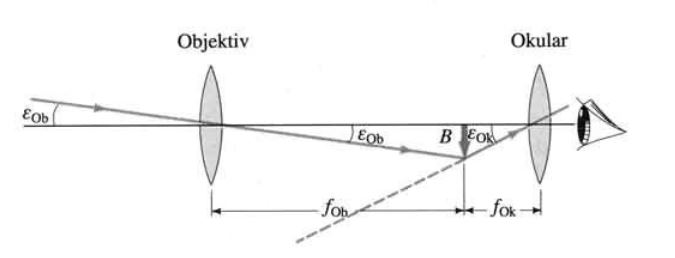
\includegraphics[scale=0.9]{Teleskop.jpg}
\end{figure}

\begin{align*}
\tan \left( \epsilon_{Ob} \right) &= - \frac{B}{f_{Ob}} \approx \epsilon_{Ob} \\
\tan \left( \epsilon_{Ok} \right) &= - \frac{B}{f_{Ok}} \approx \epsilon_{Ok}
\intertext{Vergrößerung}
\nu_T &= \frac{\epsilon_{Ok}}{\epsilon_{Ob}} = - \frac{f_{Ob}}{f_{Ok}}
\end{align*}





\section{Polarsation}

\begin{align*}
\intertext{Allgemeine Transmission:}
T_\perp &= e^{-\mu_\perp \cdot d} \\
T_\parallel &= e^{-\mu_\parallel \cdot d} 
\intertext{Dicke eine Lambdaviertelplatte:}
d &= \frac{\lambda}{4 \cdot |n_o - n_e|}
\end{align*}

Falls mit den Stokes Matrizen gerechnet werden soll bekommen wir die Tabelle dazu. Wichtig ist, das die Matrizen in umgekehrter Reihenfolge des Lichtwegs miteinander multipliziert werden.

\section{Reflexionen / Transmission}

\begin{align*}
\intertext{Die Dicke einer Antireflexschicht ist:}
d &= \frac{\lambda_0}{4 \cdot n_{AR}}
\intertext{Das erzeugt einen Gangunterschied von:}
\phi &= \frac{2 \pi}{\lambda} \cdot \frac{\lambda'}{2}
\intertext{Dabei ist $\lambda'$ die Wellenlänge gegen die die Antireflexschicht wirkt und $\lambda$ die eingestrahlte Wellenlänge.}
\end{align*}

Für die innere Transmission gilt:

\begin{align*}
T &= \frac{\left( 1 - R \right)^2 \cdot \tau}{1 - \left( R \tau \right)^2} \qquad \text{mit} \qquad \tau = e^{-Kd} 
\intertext{Für die Oberflächenreflexion gilt:}
R &= \left( \frac{n - 1}{n + 1} \right)^2
\end{align*}

Für den Brechungsindex einer Antireflexschicht auf einem Medium gilt:

\begin{align*}
n_{AR} &= \sqrt{n_{Medium}}
\end{align*}




\section{Beugung}

\begin{align*}
\intertext{Intensität am Spalt:}
I(\theta) &= \frac{\sin^2\left( \frac{\pi b \sin(\theta)}{\lambda} \right)}{\left( \frac{\pi b \sin(\theta)}{\lambda} \right)^2}
\intertext{Im ersten Minimum gilt:}
\pi &= \frac{\pi b \sin(\theta)}{\lambda}
\intertext{Für kleine Winkel gilt:}
\tan(\theta) &= \theta = \sin(\theta) = \frac{\lambda}{b}
\intertext{Wir definieren $\Delta x$ als den Abstand vom zentralen Maximum zum ersten Minumum:}
\Delta x &= L \cdot \frac{\lambda}{b}
\end{align*}

Für eine Lochblende gilt:

\begin{align*}
I(\theta) \sim \left[ \frac{2 j_1 \cdot \left( \pi d \cdot \frac{\sin(\theta)}{\lambda} \right)}{\pi d \frac{\sin(\theta)}{\lambda}} \right]^2
\intertext{Der erste dunkle Ring entspricht nun der ersten Nullstelle von $j_1$. Aus der Vorlesund wissen wir das dies bei $x = 1,22 \pi$ der Fall ist:}
1,22 \pi &= \pi d \cdot \frac{\sin(\theta)}{\lambda} \\
\Leftrightarrow \sin(\theta) &= 1,22 \cdot \frac{\lambda}{d} \approx \theta
\end{align*}

Dabei ist $d$ der Durchmesser des Lochs.













\end{document}